
\documentclass[conference]{IEEEtran}

\input epsf
\usepackage{graphicx}
\usepackage{float}
\hyphenation{}
\usepackage{mathrsfs}
\usepackage{amssymb}
\usepackage{amsmath}
\begin{document}


\title{\LARGE Analysis of Adaptive Filtering Algorithms for Acoustic Echo Cancellation}


\author{\authorblockN{Himavanth Reddy}
\authorblockA{ECE Department\\ IIIT-DM Kancheepuram, India - 600127 \\esd15i014@iiitdm.ac.in}}



\maketitle

\begin{abstract}
This paper presents an attempt to apply an adaptive filtering algorithm in order to overcome the echo generated in acoustic systems. The paper also presents a comparison between multiple adaptive algorithms in their ability to attenuate the echo in the system
\end{abstract}

\hspace{0.25em}
\IEEEoverridecommandlockouts

\begin{keywords}
Acoustic Echo Cancellation, Adaptive Algorithms, FDAF, LMS, Echo Return Loss Cancellation, Fast Fourier Transform (FFT)
\end{keywords}
\IEEEpeerreviewmaketitle


\section{Introduction}
Acoustic echo cancellation (AEC) is generally necessary in full-duplex communication scenarios where loudspeaker echoes should be removed from a microphone signal. This is necessary for teleconferences where the microphone signal is sent to far-end communication partners who may be disturbed when hearing their own voices. Adaptive filters designed for acoustic echo cancellation schemes are confronted with several difficulties. First, the number of taps needed to model the impulse response of an acoustic echo path shall be very large. Moreover, non stationary signals such as speech signals are highly correlated also the signal picked up by the microphone is corrupted by the near-end speech, and by the ambient noise. Dealing with long impulse responses, and designing adaptive filtering algorithms for highly correlated speech signals, has led to many time domain and frequency domain algorithms developed. Here we have simulated few adaptive filtering algorithms and compared them from the point of view of the performance parameter i.e. echo return loss enhancement, by varying step size.

\section{Objectives of this Project}
\begin{enumerate}
    \item Apply Frequency Domain Adaptive Filtering (FDAF) to eliminate echo in the system
    \item Compare the performance of FDAF with the well known Least Means Square (LMS) algorithm
\end{enumerate}

\section{Algorithms}
\subsection{LMS Algorithm}
This algorithm adapts to a solution of minimizing mean-square error. This method is based on steepest-descent method. In this, the gradient of mean-squared error is found out with respect to h.\\  If $w(n)$ is the weight vector and $x(n$) is the input signal then, output $y(n)$ of the adaptive filter is given by \\$y(n) = w(n)^Tx(n)$,\\ The error signal $e(n)$ is given by \\$e(n) = d(n)-y(n)$, \\
The weight update equation is given by \\$w(n+1) = w(n) + \mu e(n) x(n)$

where $\mu$ is the step size which controls the convergence rate. If the value of $\mu$ is small, then the convergence time is more. So the selection of suitable value of step size is very important. This algorithm is very simple and only requires few numbers of additions and multiplications per iteration for an N-tap filter. It has low computational complexity and the problem of double-talk is removed. But the step size chosen during every iteration in this method is of fixed size. The computational complexity of this algorithm involves $2M$ additions and $2M+1$ multiplications.

\subsection{Frequency Domain Adaptive Filtering Algorithm}
In acoustic echo cancellation the impulse response of the system often reaches over 100ms in length. This would require an adaptive FIR filter with over 1000 coefficients. The linear convolution and the update of the adaptive filter with this length creates a significant computational burden for applications that require low power processors. Thus FFT is used to minimize the number of calculations required and therefore make the algorithm more efficient.\\

Let L be the length of the block and M be the length of tapped weight vector.\\
$A_0 = \begin{bmatrix}
u(kL)\\ u(kL+1)
\\ ...
\\ u(kL + L-1)
\end{bmatrix}, A_1 = \begin{bmatrix}
u(kL-1)\\ u(kL)
\\ ...
\\ u(kL + L-2)

\end{bmatrix}$\\

The data matrix can then be written as
\begin{center}
$\mathbf{A}(k)=\left[ \begin{array}{lllll}{\mathbf{A}_{\mathbf{0}}} & {\mathbf{A}_{1}} & {\mathbf{A}_{2}} & {\cdots} & {\mathbf{A}_{M-1}}\end{array}\right]\\ = \left[ \begin{array}{l}{\mathbf{G}(k M)} \\ {\mathbf{G}(k M+1)} \\ {\cdots} \\ {\mathbf{G}(k M+L-1}\end{array}\right]$
 \end{center}

The matrix $A(k$) is an $L*M$ matrix and length of the vector $G^T(kM)$ is M. Let the weight vector be
\begin{center}
$\hat{\mathbf{W}}(k)=\left[w_{0}(k) \quad w_{1}(k) \quad w_{2}(k) \ldots w_{L-1}(k)\right]^{T}$
\end{center}\\
Output of the filter is 
\begin{center}
$[y(k L) \quad y(k L+1) \quad y(k L+2) \ldots y(k L+L-1)]^{T}$
\end{center}
$ = \mathbf{A}(k) \hat{\mathbf{W}}(k)$ \\
For individual element,
\begin{center}
$y(k L)=G(k M) \hat{W}(k)$ \\ $y(kL+1)=G(k M+1) \hat{W}(k)$ \\ $.............. $ \\ $ y(kL+i)=G(k M+i) \hat{W}(k) \\ =\left[w_{0}(k) \quad w_{1}(k) \quad w_{2}(k) \ldots \quad \ldots \quad \ldots \quad \ldots w_{L-1}(k)\right] * \left[ \begin{array}{c}{u(k L+i)} \\ {u(k L+i-1)} \\ {u(k L+i-2)} \\ {\vdots} \\ {u(k L+i+M-1)}\end{array}\right]$ \\ $=\sum_{j=0}^{M-1} w_{j}(k) . u(k L+i-j)$
\end{center}
Let the desired response of $(kL+i)-th$  element is $d(kL+i)$. Therefore, the error signal is \\
\begin{center}
$e(k L+i)=d(k L+i)-y(k L+i)$
\end{center}

In matrix form,\\
$\left[ \begin{array}{l}{d(k L)} \\ {d(k L+1)} \\ {d(k L+2)} \\ {\cdots} \\ {\dots} \\ {\cdots} \\ {d(k L+L-1)}\end{array}\right] - \left[ \begin{array}{l}{y(k L)} \\ {y(k L+1)} \\ {y(k L+2)} \\ {\cdots} \\ {\dots} \\ {\cdots} \\ {y(k L+L-1)}\end{array}\right] = \left[ \begin{array}{l}{e(k L)} \\ {e(k L+1)} \\ {e(k L+2)} \\ {\cdots} \\ {\dots} \\ {\cdots} \\ {e(k L+L-1)}\end{array}\right] = \textbf{e(k)}$\\

The cross correlation vector is
\begin{center}
$\mathbf{\Phi}(k)=\mathbf{A}^{T}(k) \mathbf{e}(k)$
\end{center}

The update equation of the weight vector can be written as
\begin{center}
$\hat{\mathbf{W}}(k+1)=\hat{\mathbf{W}}(k)+\mu \mathbf{\Phi}(k)$
\end{center}
where $\mu$ is the step-size parameter.\\
Now using $\hat{\mathbf{W}}(k+1)$ we have\\
$\begin{array}{l}{[y(k L+L) y(k L+L+1) y(k L+L+2) \ldots y(k L+2 L-1)]^{T}} \\ {\quad=\mathbf{A}(k+1) . \hat{\mathbf{W}}(k+1)}\end{array}$\\ \\
The updated error matrix is \\
$\left[ \begin{array}{l}{d(k L+L)} \\ {d(k L+L+1)} \\ {d(k L+L+2)} \\ {\cdots} \\ {\cdots} \\ {\cdots} \\ {d(k L+2 L-1)}\end{array}\right] - \left[ \begin{array}{l}{y(k L+L)} \\ {y(k L+L+1)} \\ {y(k L+L+2)} \\ {\cdots} \\ {\cdots} \\ {y(k L+2 L-1)}\end{array}\right] = \left[ \begin{array}{l}{e(k L+L)} \\ {e(k L+L+1)} \\ {e(k L+L+2)} \\ {\cdots} \\ {\cdots} \\ {\cdots} \\ {e(k L+2 L-1)}\end{array}\right] = \textbf{e(k+1)}$

The updated cross correlation vector and the weight vector are respectively as
\begin{center}
$\mathbf{\Phi}(k+1)=\mathbf{A}^{T}(k+1) \mathbf{e}(k+1)$
\end{center}
and
\begin{center}
$\hat{\mathbf{W}}(k+2)=\hat{\mathbf{W}}(k+1)+\mu \mathbf{\Phi}(k+1)$
\end{center}
Similarly,\\
$\begin{array}{c}{[y(k L+i L) y(k L+i L+1) y(k L+i L+2) \ldots} \\ {y(k L+(i+1) L-1) ]^{T}=\mathbf{A}(k+i) \cdot \hat{\mathbf{w}}(k+i)}\end{array}$\\
Let\\
$\left[ \begin{array}{l}{d(k L+i L)} \\ {d(k L+i L+1)} \\ {d(k L+i L+2)} \\ {\cdots} \\ {\ldots} \\ {\ldots} \\ {d(k L+(i+1) L-1)}\end{array}\right] - \left[ \begin{array}{l}{y(k L+i L)} \\ {y(k L+i L+1)} \\ {y(k L+i L+2)} \\ {\cdots} \\ {\ldots} \\ {\ldots} \\ {y(k L+(i+1) L-1)}\end{array}\right] = \left[ \begin{array}{l}{e(k L+i L)} \\ {e(k L+i L+1)} \\ {e(k L+i L+2)} \\ {\cdots} \\ {\ldots} \\ {\ldots} \\ {e(k L+(i+1) L-1)}\end{array}\right] = \textbf{e(k+i)}$ \\

In generalized form,\\
\begin{center}
$\mathbf{\Phi}(k+i)=\mathbf{A}^{T}(k+i) \mathbf{e}(k+i)$
\end{center}
and
\begin{center}
$\hat{\mathbf{W}}(k+i+1)=\hat{\mathbf{W}}(k+i)+\mu \Phi(k+i)$
\end{center}
In overlap-save method $N=2M$ point FFT is used and the
size of the filter of $M$ tap weights.\\
Input signal in n domain is express as, $[(k-1)th$ block, $kth$ block], where the $(k-1)th$ block is \\
$\begin{bmatrix}
u(kL-L) & u(kL-L-1)   & ...  & u(kL-2M+1)\\ 
u(kL-L+1) & u(kL-L)   & ...  & u(kL-L-2M+2) \\ 
 ..& .. & .. & .. \\ 
u(kL-1) & u(kL-2) & ...  & u(kL-2M)
\end{bmatrix}$\\ \\

And the k-th block is \\
$\begin{bmatrix}
u(kL) & u(kL-1)  & ...  & u(kL-2M+1)\\ 
u(kL+1) & u(kL)   & ...  & u(kL-2M+2) \\ 
 ..& .. & .. & .. \\ 
u(kL+M-1) & u(kL+M-2)  & ...  & u(kL-M)
\end{bmatrix}$ \\ \\
Input signal in k domain,\\ 
$\mathbf{U}(k)=\operatorname{diag}(F F T[(k-1) t h \text { block, } k t h \text { block }])$\\
an $N*N$ matrix. The initial weight in k domain is a $1 * N$
vector: \\
$\hat{\mathbf{W}}(k)=F F T \left[ \begin{array}{l}{\hat{\mathbf{w}}(k)} \\ {\mathbf{O}}\end{array}\right]$ \\

Here $\hat{\mathbf{w}}(k)$ is tap-weight vector (in n domain) of length M
and \textbf{O} is a null vector of length M. \\ \\
Output signal of the filter in k domain is \\
$\hat{\mathbf{y}}(k)$ = Last $M$ elements of IFFT[$U(k)\hat{\mathbf{W}}(k)$]\\
The desired response vector,\\
$\mathbf{d}(k)=\left[d(k M), d(k M+1), \ldots d(k M+M-1]^{T}\right.$ \\ \\
Error signal vector in n domain,\\
$\begin{aligned} \mathbf{e}(k) &=[e(k M), e(k M+1), \ldots& \ldots, e(k M+M-1]^{T} \\ &=\mathbf{d}(k)-\mathbf{y}(k) \end{aligned}$ \\
The error signal in the frequency domain is
\begin{center}
$\mathbf{E}(k)=F F T \left[ \begin{array}{l}{\mathbf{O}} \\ {\mathbf{e}(k)}\end{array}\right]$
 \end{center} 
The cross-correlation vector is\\
$\phi(k)$ = First M elements of IFFT[$U^H(k)E(k)$]\\
Thus, the updated tap-weights can be written as, 
\begin{center}
$\hat{\mathbf{W}}(k+1)=\hat{\mathbf{W}}(k)+\mu F F T \left[ \begin{array}{c}{\varphi(k)} \\ {\mathbf{O}}\end{array}\right]$
\end{center}

FDAF provide several advantages over its time domain counterpart. Besides being able to perform the filter convolution by a multiplication in frequency domain, also the length of the adaptive filter are effectively decimated by the transformation. Thus, the computational complexity of the adaptive algorithm is reduced. In addition, to reduced computational complexity, FDAF can also provide an increased convergence speed. This is a result from the decreased eigenvalue spread of the auto-correlation matrix of the signals in the filter update.\\

These advantages of the FDAF ultimately come with a tradeoff. The main costs of FDAF are increased latency and an increased memory requirement. The latency cost comes from the need to delay the desired signal (or microphone signal in echo cancellation) by the delay through the frequency domain filter. This results in an increased memory storage over time domain approaches because both the excitation and desired signals need to be stored.\\
The total computational complexity of FDAF is given by: $10M log(M) + 26M$

\section{Implementation}
The entire system is simulated in MATLAB with the help of the DSP toolbox. Initially, a room impulse response is generated which acts as the echo path.microphone which is called as near end speech signal. A voice travels out the loudspeaker, bounces around in the room, and this voice is picked up by the system's microphone, this voice signal is called as far end speech signal. The microphone signal contains both the near end and far end speech signals and some additional noise. The adaptive algorithm is then applied on the microphone signal in order to attenuate the noise and obtain the original near end speech signal. The adaptive filters are chosen to be of length 2048 and the input signal is sampled at a rate of 16000Hz

\section{Performance Parameters}
The performance parameter which is used here for the performance evaluation of different AEC Algorithms is known as Echo Return Loss Enhancement (ERLE).\\ 

It is a smoothed measure of the amount (in dB) that the echo has been attenuated. It is mathematically defined as \\
	\begin{center}
	ERLE(dB) $= 10log_{10}{\frac{d^2(n)}{e^2(n)}}$
	\end{center}
Where,\\
$d(n)$ is the far-end echoed signal \\
$e(n)$ is the residual echo after cancellation

\section{Results}
The results of LMS and FDAF are compared, each with 2 different values of step sizes
	\begin{figure}
		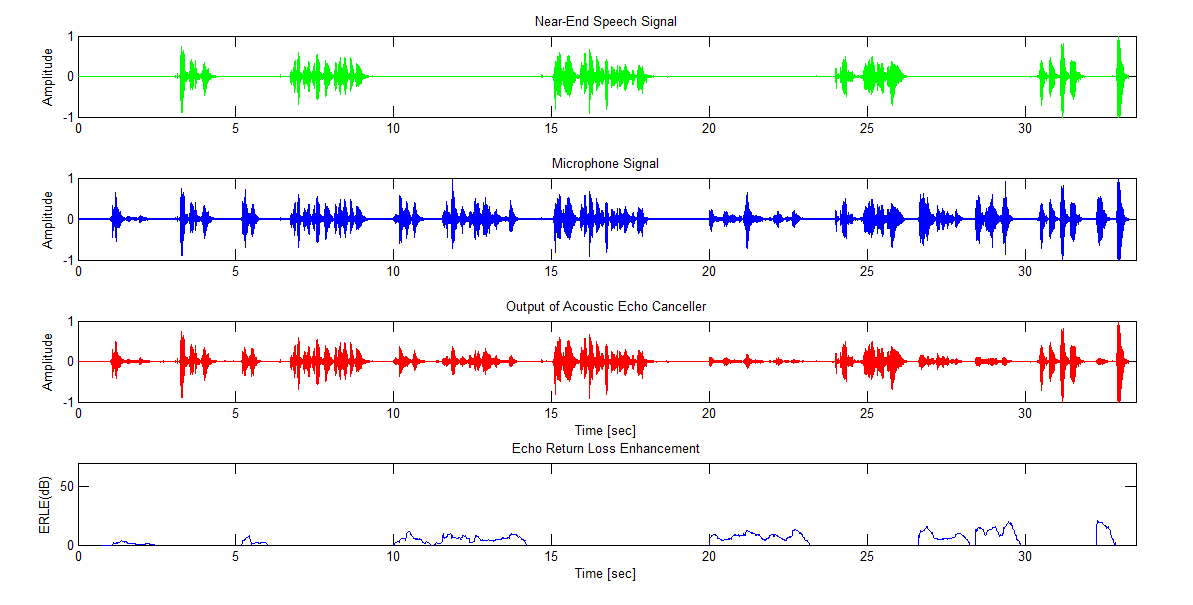
\includegraphics[height=6cm, width=8cm]{LMS_Result_5e-2}
		\caption{Results with LMS algorithm, Step size = 0.05}
	\end{figure}
	
	\begin{figure}
		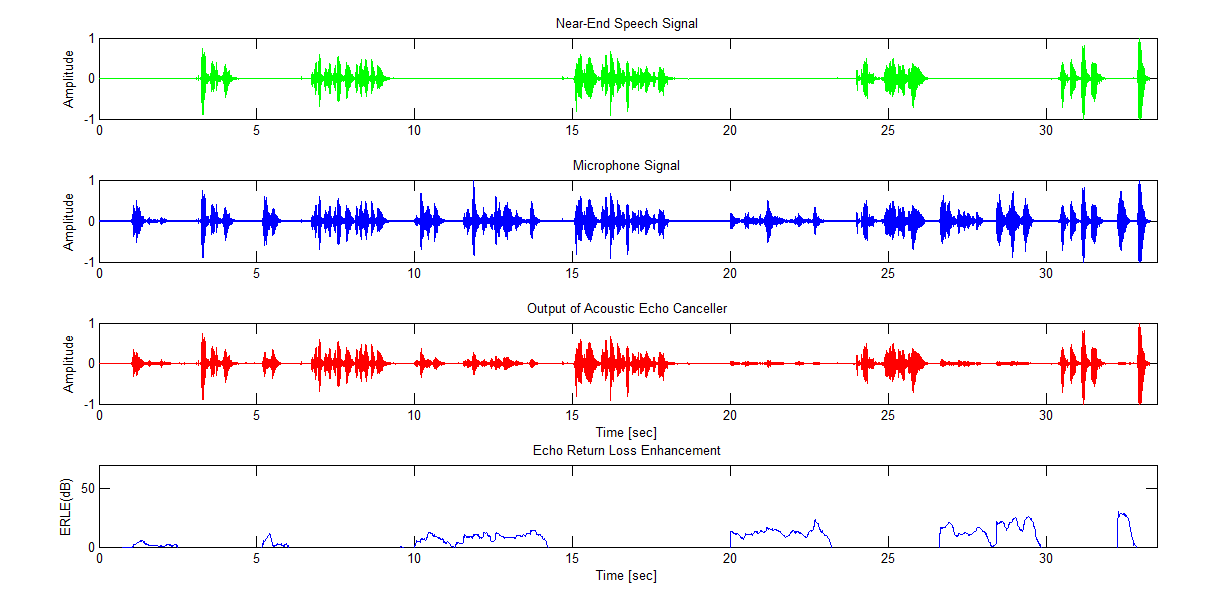
\includegraphics[height=6cm, width=8cm]{LMS_Result_13e-2}
		\caption{Results with LMS algorithm, Step size = 0.13}
	\end{figure}
	
	\begin{figure}
		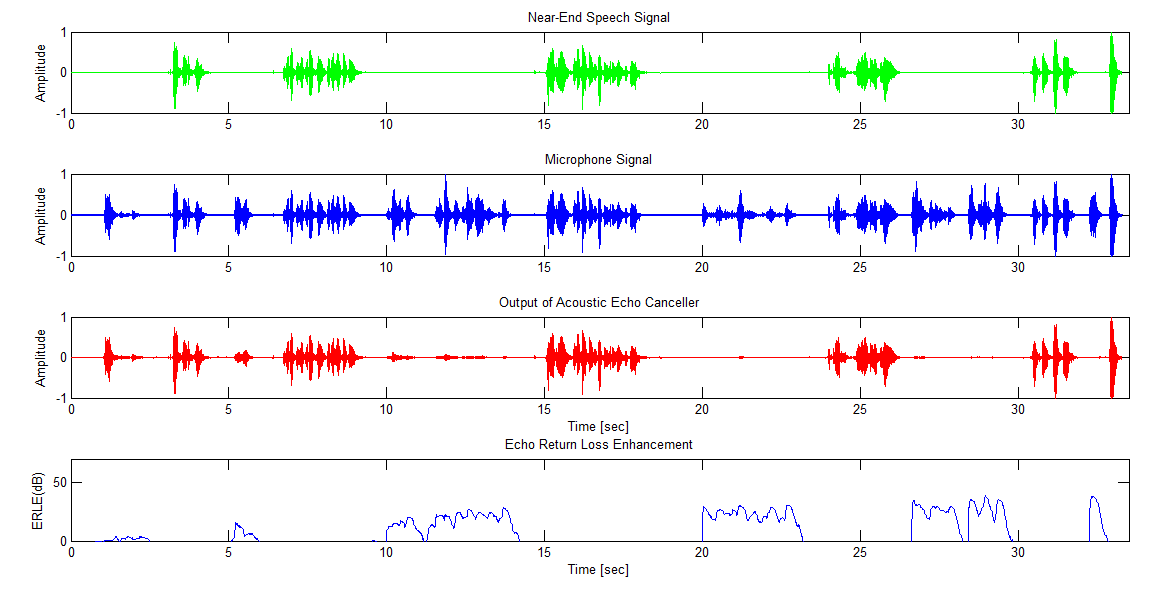
\includegraphics[height=6cm, width=8cm]{FDAF_Result}
		\caption{Results with FDAF algorithm, Step size = 0.025}
	\end{figure}

	\begin{figure}
		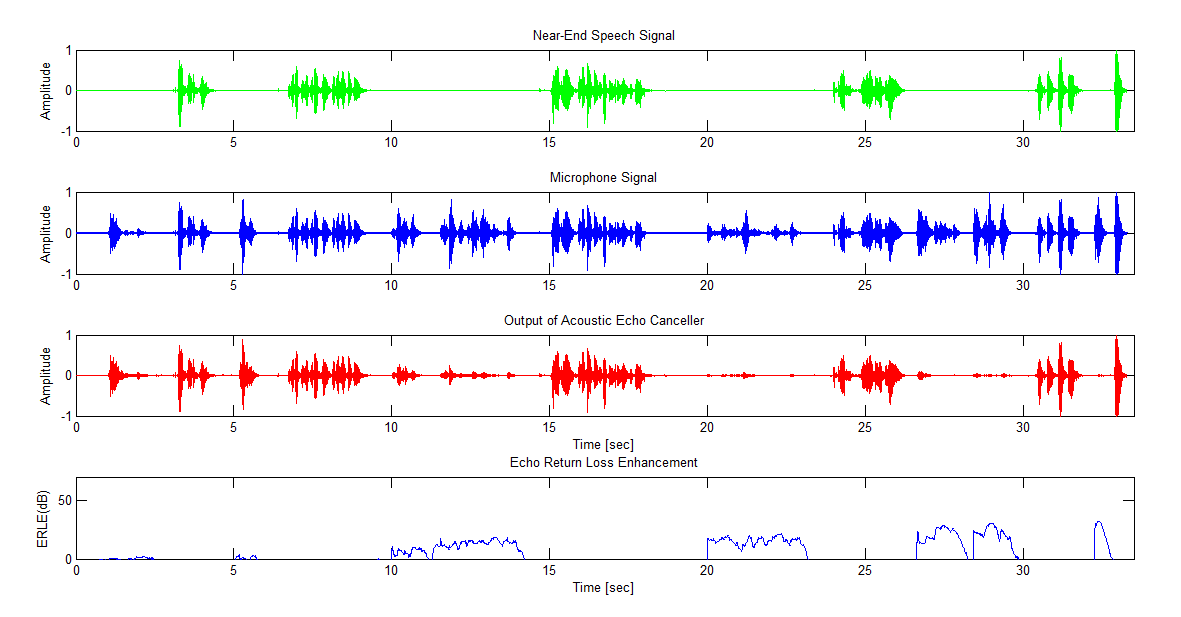
\includegraphics[height=6cm, width=8cm]{FDAF_Result_5e-2}
		\caption{Results with FDAF algorithm, Step size = 0.05}
	\end{figure}


\section{Conclusion}
Based on the simulation results we can see that the FDAF algorithm provides results that are significantly better than its LMS counterpart. This is primarily because of the long impulse responses and high number of filter coefficients of the system which are effectively handled by FDAF but at the cost of latency and memory requirement.\\
Algorithms such as Partition Block FDAF are known to show better performance compared to FDAF in terms of Echo Return Loss Enhancement

\begin{thebibliography}{1}
\bibitem{Paleo} 
Paleologu, Constantin and Ciochin{\u{a}}, Silviu and Benesty, Jacob
and Grant, Steven L. \textit{An overview on optimized NLMS algorithms for acoustic echo cancellation}. 
EURASIP Journal on Advances in Signal Processing 2015. Nov 19, 2015

\bibitem{Haykin} 
Simon Haykin. \textit{Adaptive Filter Theory, 4th edition}. 
Upper Saddle River, NJ: Prentice-Hall 2002

\bibitem{Patil} 
AP Patil and MR Patil \textit{Performance analysis of Adaptive Filtering Algorithms for Acoustic Echo Cancellation}. 
International Journal of Engineering Research and Technology, Vol.7, Issue.08, Aug 2018.

\bibitem{Kamarudin} 
Kamarudin, Noraziahtulhidayu and Al-Haddad, S. A. R. and Abushariah, Mohammad A. M. and Hashim, Shaiful Jahari and Hassan, Abd Rauf Bin \textit{Acoustic echo cancellation using adaptive filtering algorithms for Quranic accents (Qiraat) identification}. 
International Journal of Speech Technology, Vol.19, No.2 , Jun 2016, Pages 393-405
\end{thebibliography}
\smallskip
\end{document}